% -*- coding: utf8 -*-

\defaultfont
\chapter*{哈尔滨工业大学硕博士学位论文\\开题报告模板~\version~版}
% 或 不要题目
%\vspace*{-10pt}

%%%%%%%%%%%%%%%%

\section{课题背景及意义}
\label{Introduction:background}


\LaTeX~由于具有排版美观、对公式和图表的处理能力强大以及跨平台通用性强等优势,
使得它在科技排版中的应用越来越广泛。


在哈尔滨工业大学硕博士学位论文模板(SVN仓库版本150,介于1.8rc1和目前未发布的1.8rc2之间)的基础上,LaTeX@lilac
制作了工大的研究生硕博士开题报告模板,并加入到PlutoThesis项目中,和其他管理员一块维护。

\section{入门知识}
\label{sec:learningknowledge}
考虑到不少同学没有接触过~\LaTeX{},为了少走弯路,快速上手,尽快学会~\LaTeX{}的基本使用方法,
从而把更多的时间投入到论文的写作过程中,更专注于论文的内容,特增加一节介绍~\LaTeX 的基本知识,
推荐一些文档资料,及常用的编辑技巧等内容。

\subsection{什么是\LaTeX{}}
\label{sec:whatislatex}
   \TeX/\LaTeX 是一套功能强大、排版完美的开放源程序的免费办公排版软件。

    对多种操作系统,包括~Microsoft Windows、 Unix类~(如:Solaris、 Linux 等)、 %\CJKglue \CJKglue \CJKglue
以及~Mac OS X 均供有相应的运行版本,其名字也不尽相同,其发展过程类似于基于~linux 内
核的众多~linux 操作系统的发展过程。

   在~Windows 下最常用的是~\href{http://www.miktex.org}{MikTeX} 及其衍生出来的套装。Linux 下现在最常用并且持续更新的是
TeXlive(跨平台,某些版本也可用在windows下),另一个编译系统~teTeX 最近停止了维护。

  在MikTeX基础上,\href{http://www.ctex.org}{CTeX} 的~Aloft 站长加入了中文输入输出支持,配置了~CTeX 中文套
装,安装即用,免去了用户的配置之苦,推荐中文用户入门使用。

   与所见即所得~(WYSIWYG,What You See Is What You Get) 的~Microsoft Office
软件相比,它的特点是:
\begin{itemize}
      \item 所想即所得~(WYSTWYG,What You Think Is What You Get),让你更专注
于论文的思路贯通而不是繁杂的格式要求,更适合排版科技论文;

论文的思路贯通而不是繁杂的格式要求,更适合排版科技论文;论文的思路贯通而不是繁杂的格式要求,更适合排版科技论文;
论文的思路贯通而不是繁杂的格式要求,更适合排版科技论文;
      \item 控制格式方便,键盘输入快捷,数学公式输入排版方便,输出精美;
      \item 纯文本文件避免了类似~MSWord 的各种格式易变、文档损坏、公式无法编辑等不稳定现象,
      也更有利于版本控制;
      \item 输出的~PDF 文件是国际文档标准,哈工大要求硕博士毕业论文提交的也是~PDF 格式;
      \item 国际期刊及会议一般都提供~\LaTeX 论文模板,使论文投稿排版更容易;
      \item 目前国内外不少高校也都具有~\LaTeX{}学位论文写作模板,使写作学位论文的排版不再是痛苦,
      而是一种享受。哈工大比较成熟的即为此模板;
      \item 制作幻灯片的~LaTeX 宏包~beamer,排版公式和输入文字一样方便,没有~PowerPoint
的那种繁琐公式和图片位置调整,众多的默认模版供选择,一个简单命令就可切换,让幻灯
片制作更轻松、专业、漂亮;
      \item  众多的文档类和宏包支持,给你的感觉是``没有你做不到的,只有你想不到的'';
      \item  对许多忠实的~TeXer 而言,\TeX/\LaTeX 已经不仅仅是一种排版软件,更成为一种信仰,
      因为它的诞生及其发展本身就是一段趋向完美的传奇。
\end{itemize}

    很多人都对~\LaTeX{} 做过介绍,你可以从紫丁香的TeX版编号为~ 1 的帖子往后翻上几页看看。校内的
    \url{ftp://202.118.224.241/software/Science/TeX&LaTeX/TeX\%20documents} 上也有几个幻灯片对它进行了介绍。
    本文作者反复修改多次,最后决定推荐网站~\href{http://zzg34b.w3.c361.com/index.htm}{LaTeX编辑部} 上的几篇文章,快速全面了解它。
   \begin{itemize}
     \item  \href{http://learn.tsinghua.edu.cn:8080/2001315450/tex_frame.html}{TeX简介}:我们使用的~\LaTeX 系统的基础;
     \item \href{http://zzg34b.w3.c361.com/homepage/TeXvirtue.htm}{TeX的优缺点}: 它趋向完美,但是还不是十全十美;
     \item \href{http://zzg34b.w3.c361.com/homepage/LaTeXbring.htm}{LaTeX的产生}:我们日常接触最多的是它;
     \item \href{http://zzg34b.w3.c361.com/homepage/compareWord.htm}{LaTeX应用情况}:国内外的情况,现在国内是使用者越来越多。
     \item \href{http://zzg34b.w3.c361.com/homepage/compareWord.htm}{与Word相比较}:对于我们用的软件~word和~LaTeX,二者各有优点和缺点,不要陷入很偏执的观点中,这是一篇比较客观的文章。
     \item \href{http://zzg34b.w3.c361.com/homepage/KnuthResume.htm}{Knuth 教授简历}:底层内核~ \TeX 的作者~ Donald Knuth (高德纳)的介绍,富有传奇色彩;
     \item \href{http://zzg34b.w3.c361.com/homepage/LamportResume.htm}{Lamport 博士简历}: \LaTeX 的作者~Lamport,由于他的努力,才让~\LaTeX 使用简单很多,风靡科技界;
   \end{itemize}

\subsection{推荐软件及其下载}
\label{sec:latexsoftware}
\begin{figure}[htbp]
\centering
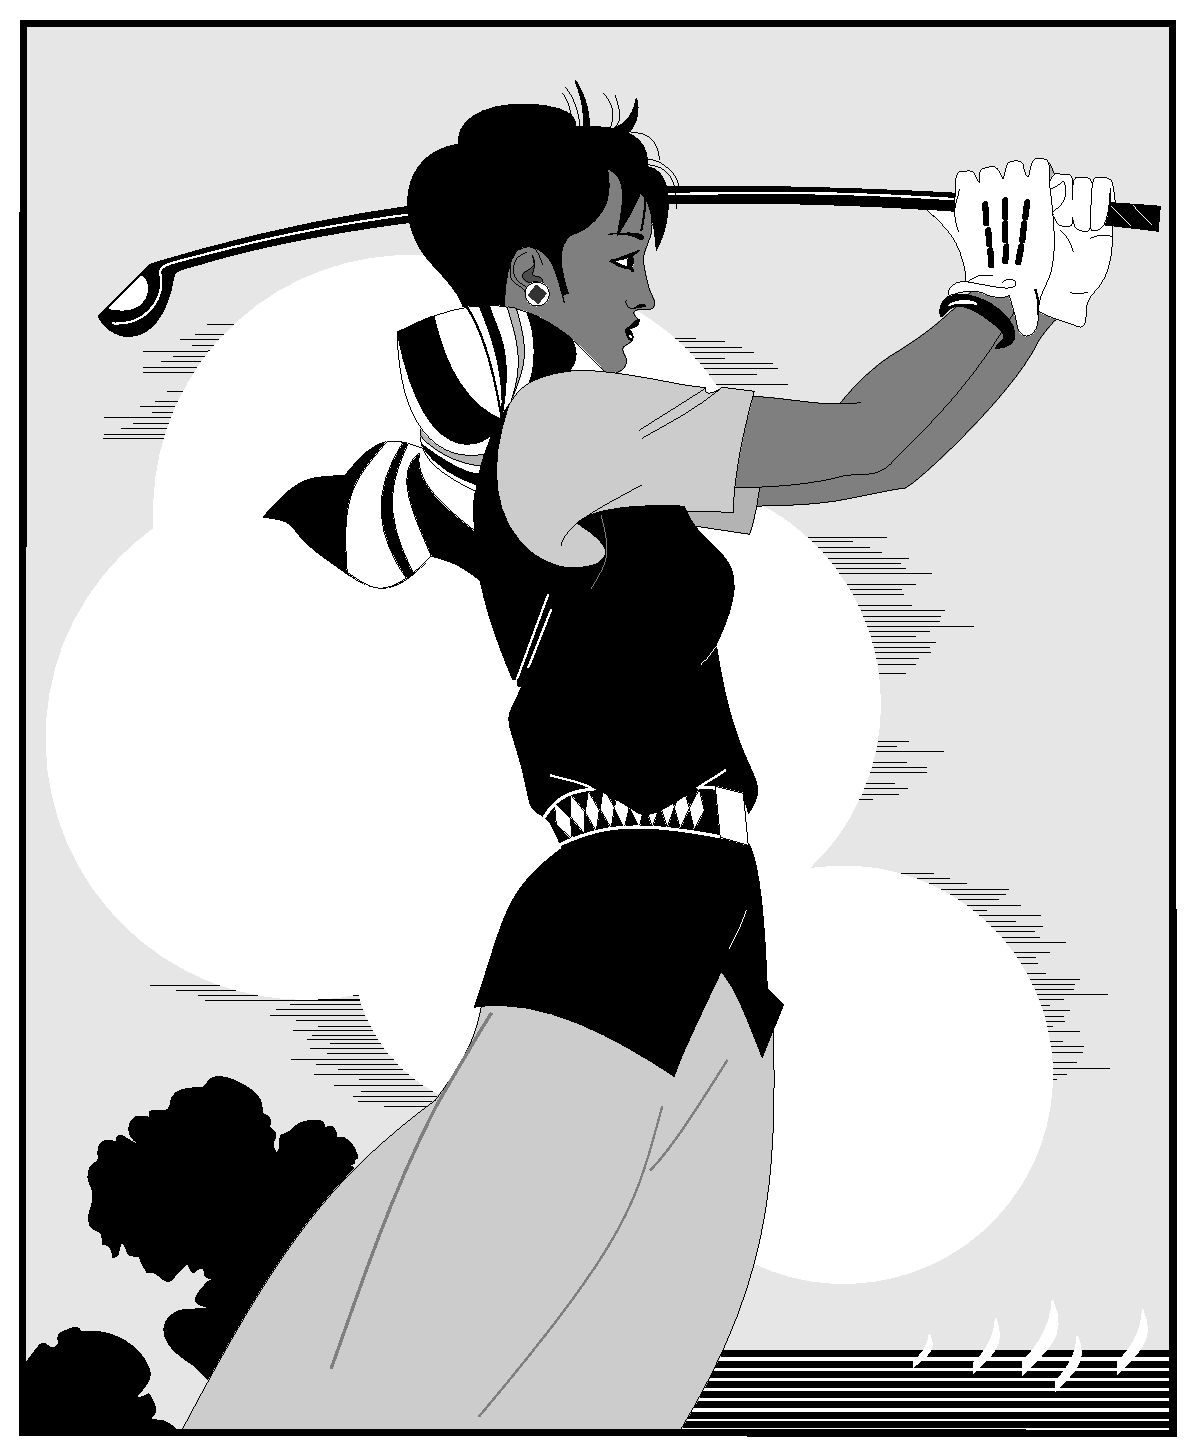
\includegraphics[width = 0.4\textwidth]{golfer}
\FigCaption{打高尔夫球的人打高尔夫球的人打高尔打高尔夫球的人打高尔夫球的人打高尔夫球的人打高尔夫球的人打高尔夫球的人}
\label{Figure:Tricks:Example12}
\end{figure}
对于新手,Windows 下只推荐免费的~CTeX 套装,因为丝毫不需要自己配置,安装后就可以使用。
哈工大校园网用户可以从~ \url{ftp://202.118.224.241/software/Science/TeX&LaTeX/CTex/} 下载~
CTeX-2.4.5-8-Full.exe 和~ CTeX-Fonts-2.4.4.exe,先安装套装系统,然后安装字体。非校园网用户
可以从~ \href{http://www.ctex.org}{CTeX的官方网站} 下载这两个文件。

\subsection{推荐的入门资料}

如果你是第一次接触~ LaTeX,那么安装~ CTeX 之后,不要直接打开编辑软件~WinEdt 进行操作,因为现在你对这个软件了解还较少,会无所适从。请从~ Windows
系统的开始~ $\rightarrow$ 程序~ $\rightarrow$ 中文 TeX 套装~ $\rightarrow$ help $\rightarrow$
看到文档了吧,我们建议的顺序是:首先打开~ CTeX FAQ,从头读到''新手入门''这一节,然后
从同一目录下打开~ LShort-cn 文件,从头到尾认真浏览一遍,不用尝试记住所有的命令,
只要了解~ LaTeX 的特点,对每一部份有一个感性认识就可以。以后你还可以回头来翻看相关命令。
然后把 ~CTeX FAQ 浏览完毕,在这个过程中,可以尝试去练习排版一些文档,查看编译效果(具体~ WinEdt 编译
方法请看后面的节 \ref{sec:winedttricks})。

你会留意到还有两个文档~PDF: latex2e 插图指南和~mathematics (LaTeX 宝典 The LaTeX Companion 的~chapter8),
分别是讲插图知识和公式输入方法的,都很详细,建议也浏览一下。对于公式输入,还有一个特别值得推荐的是
\href{http://www.tug.org/tex-archive/info/math/voss/mathmode/}{mathmode 2.0},校园网用户还可以从
\href{ftp://202.118.224.241/software/Science/TeX&LaTeX/TeX documents/}{校内~FTP TeX 资料目录}下载。
%\iffalse
\begin{figure}[htbp]
\centering
\subfigure[高尔夫1]{\label{Figure:Tricks:Example2:a}
  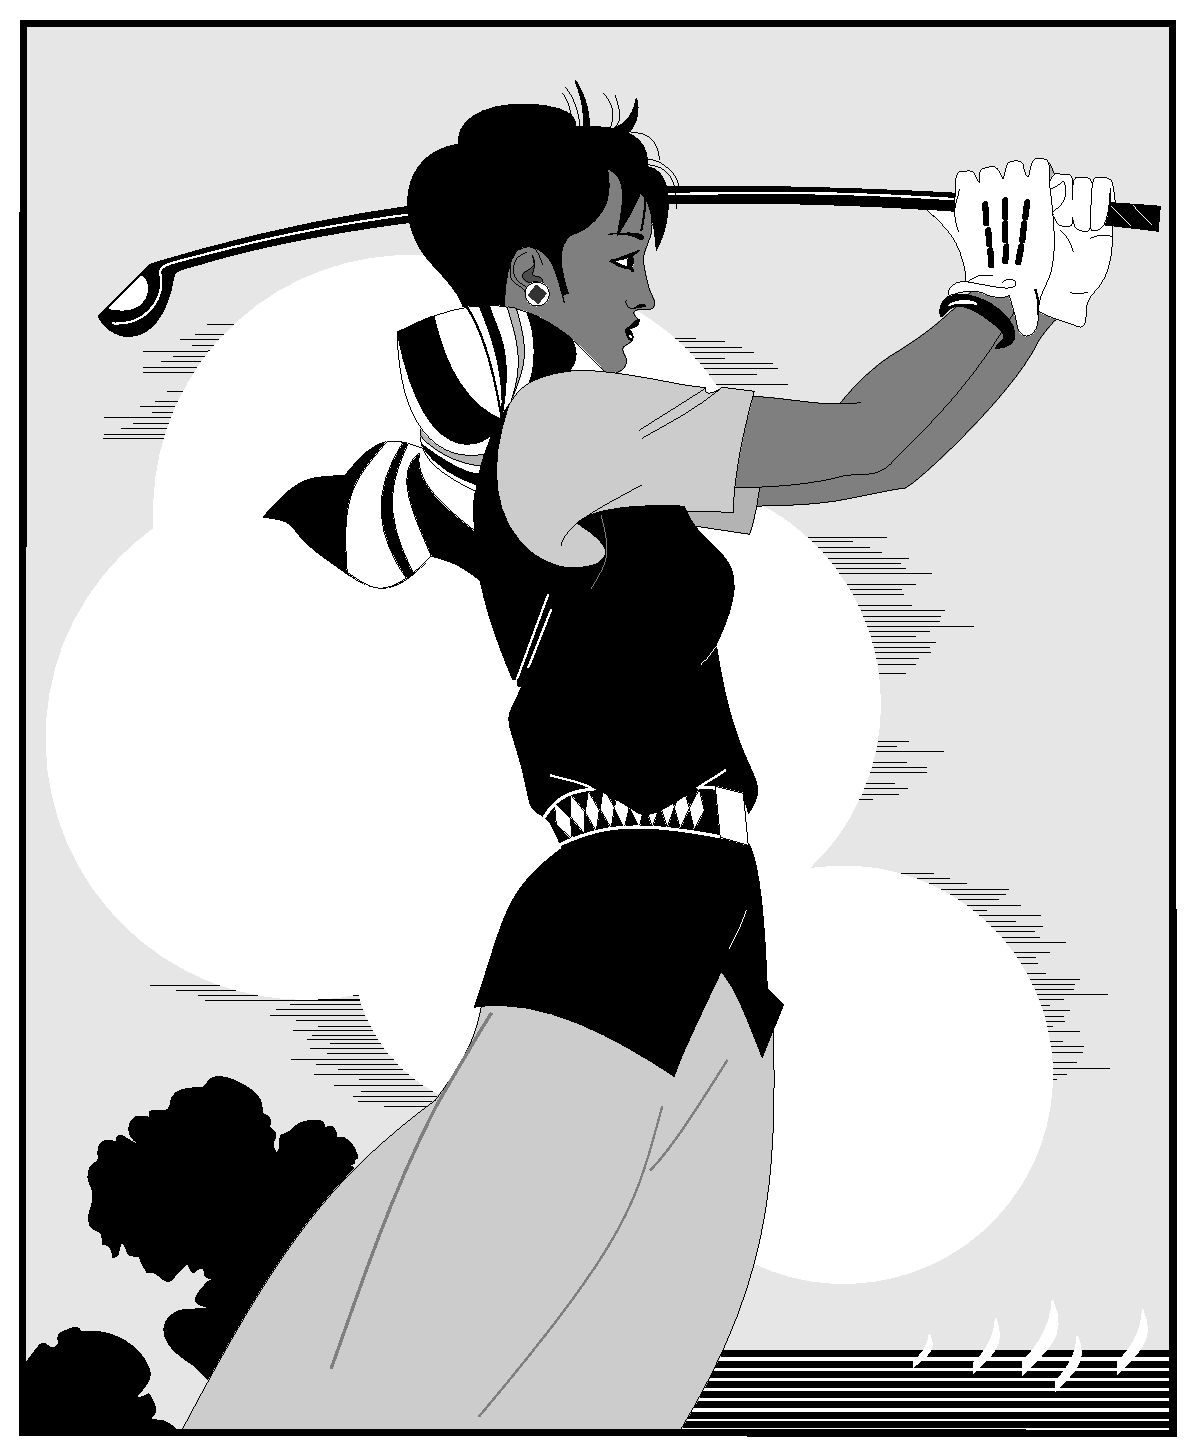
\includegraphics[width = 0.22\textwidth]{golfer}
}
\subfigure[高尔夫2]{\label{Figure:Tricks:Example2:B}
  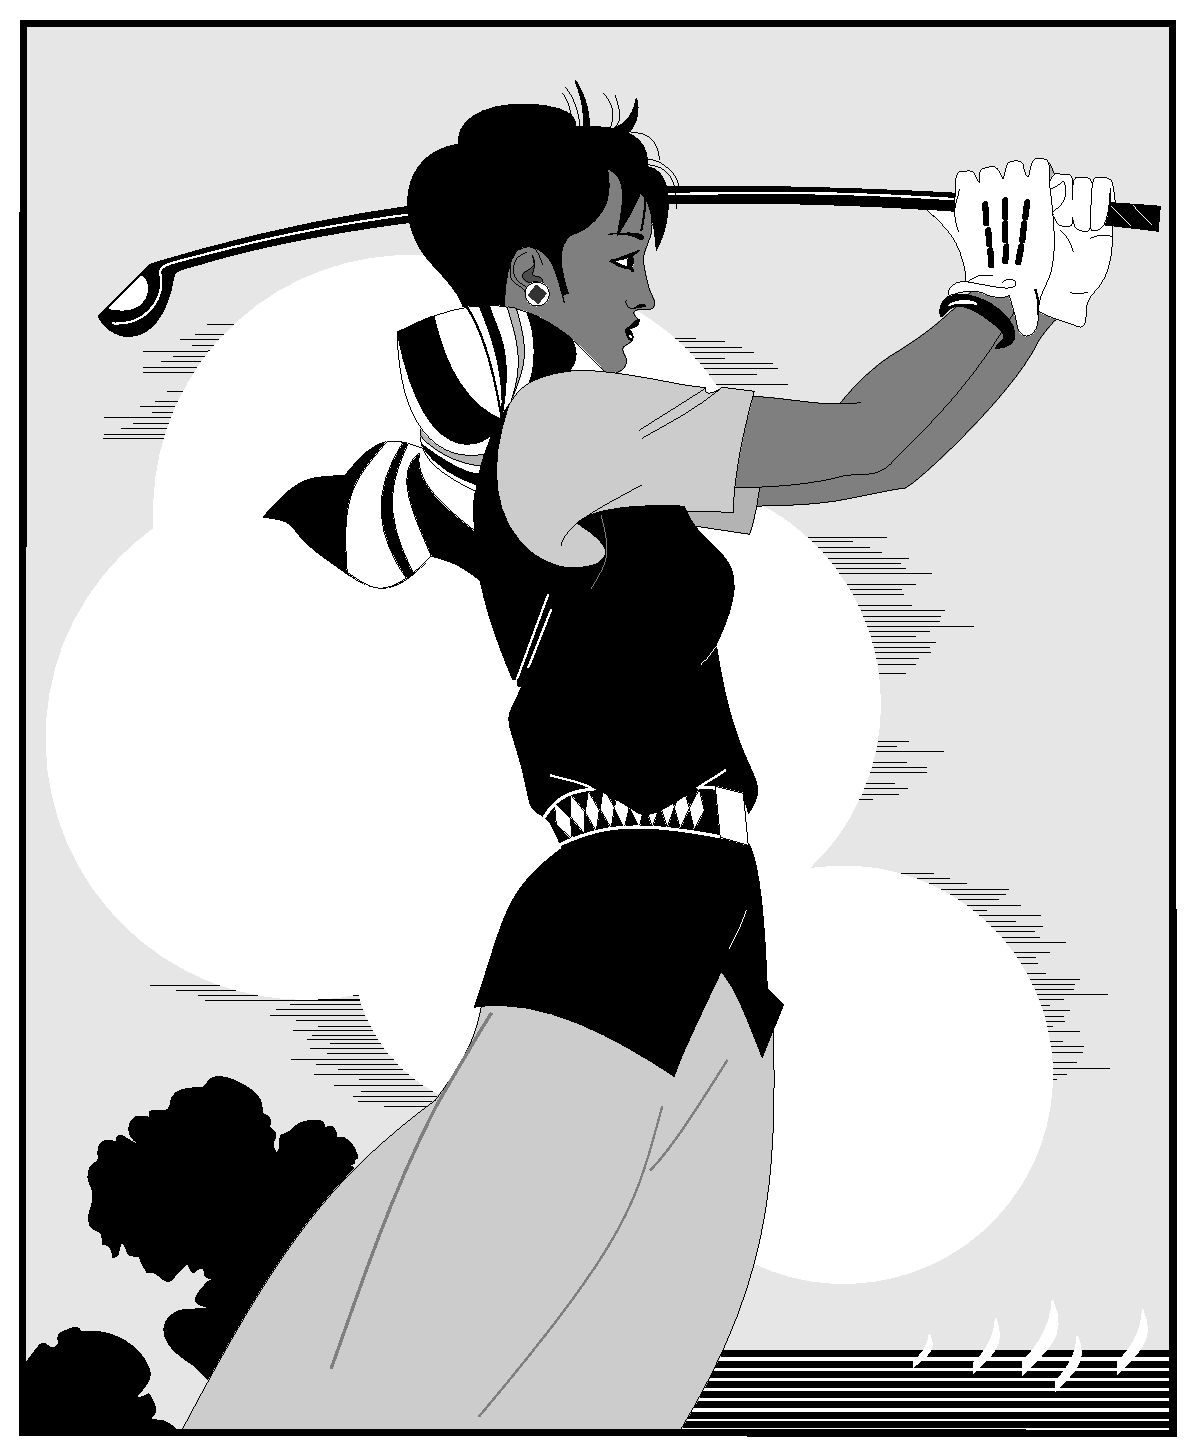
\includegraphics[width = 0.22\textwidth]{golfer}
}
\FigCaption{高尔夫}
\label{Figure:Tricks:Example2}
\end{figure}
%\fi

\begin{figure}[htbp]
\centering
\begin{minipage}{0.25\textwidth}
\centering
\subfigure[高尔夫1]{\label{Figure:Tricks:Example3:a}
  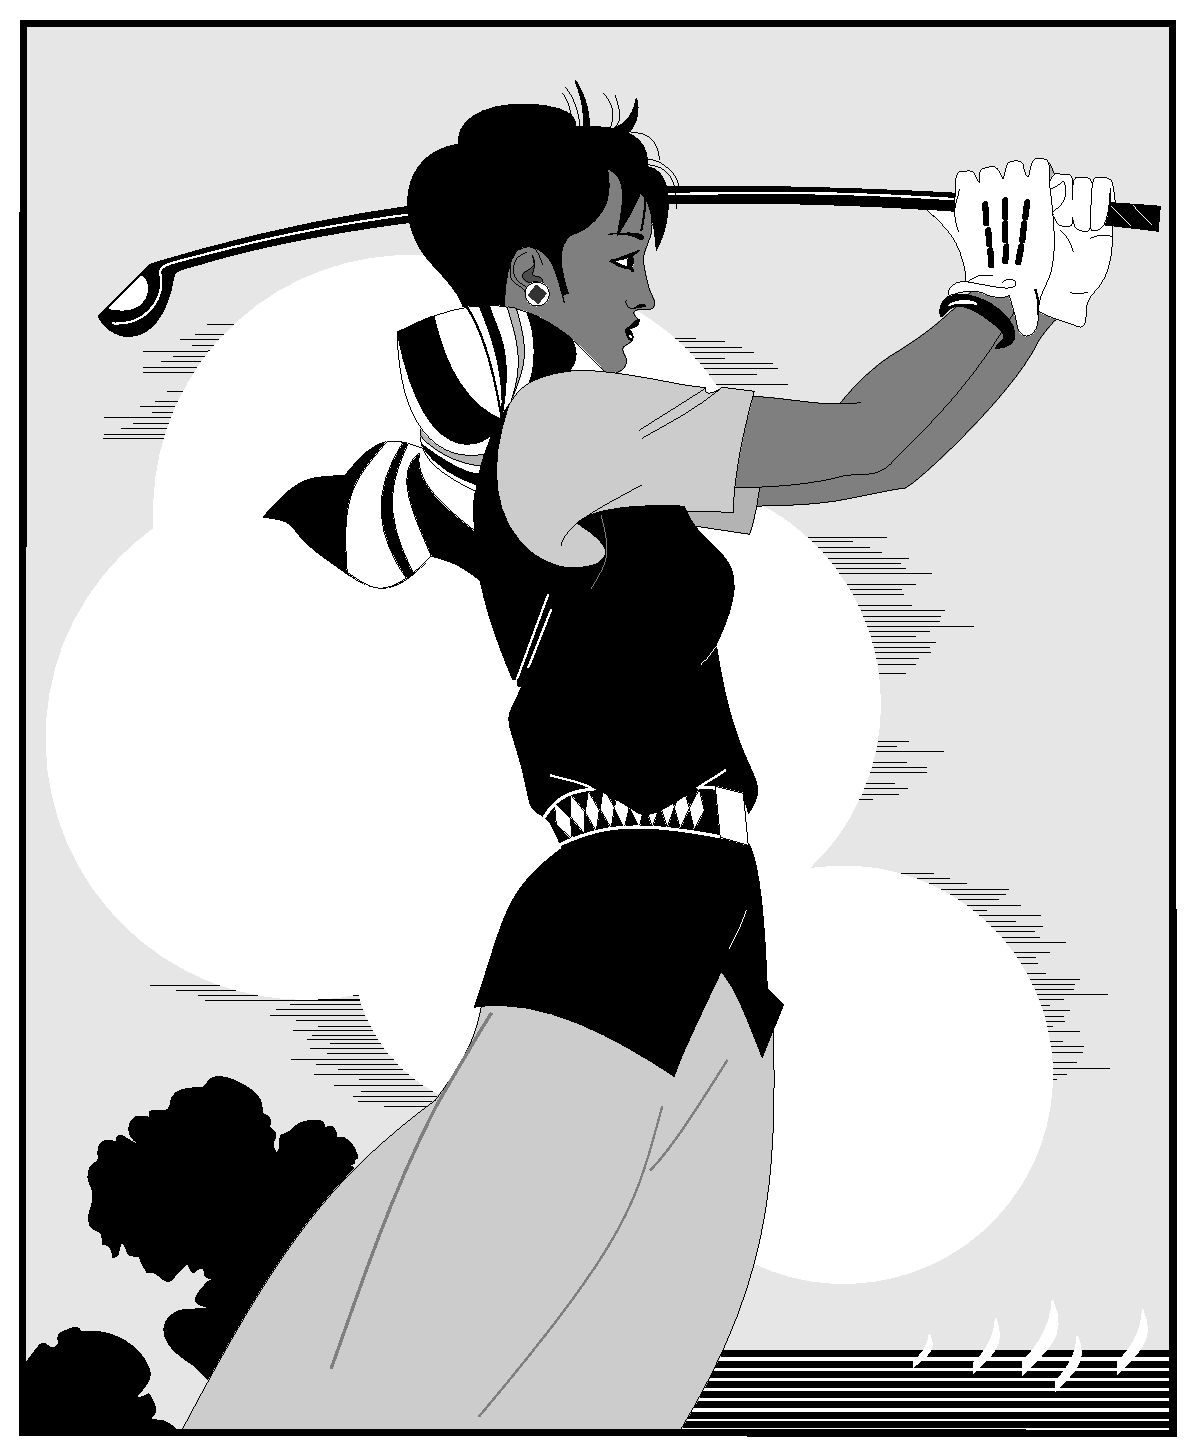
\includegraphics[width = \textwidth]{golfer}
}
\end{minipage}
\begin{minipage}{0.25\textwidth}
\centering
\subfigure[高尔夫2]{\label{Figure:Tricks:Example3:B}
  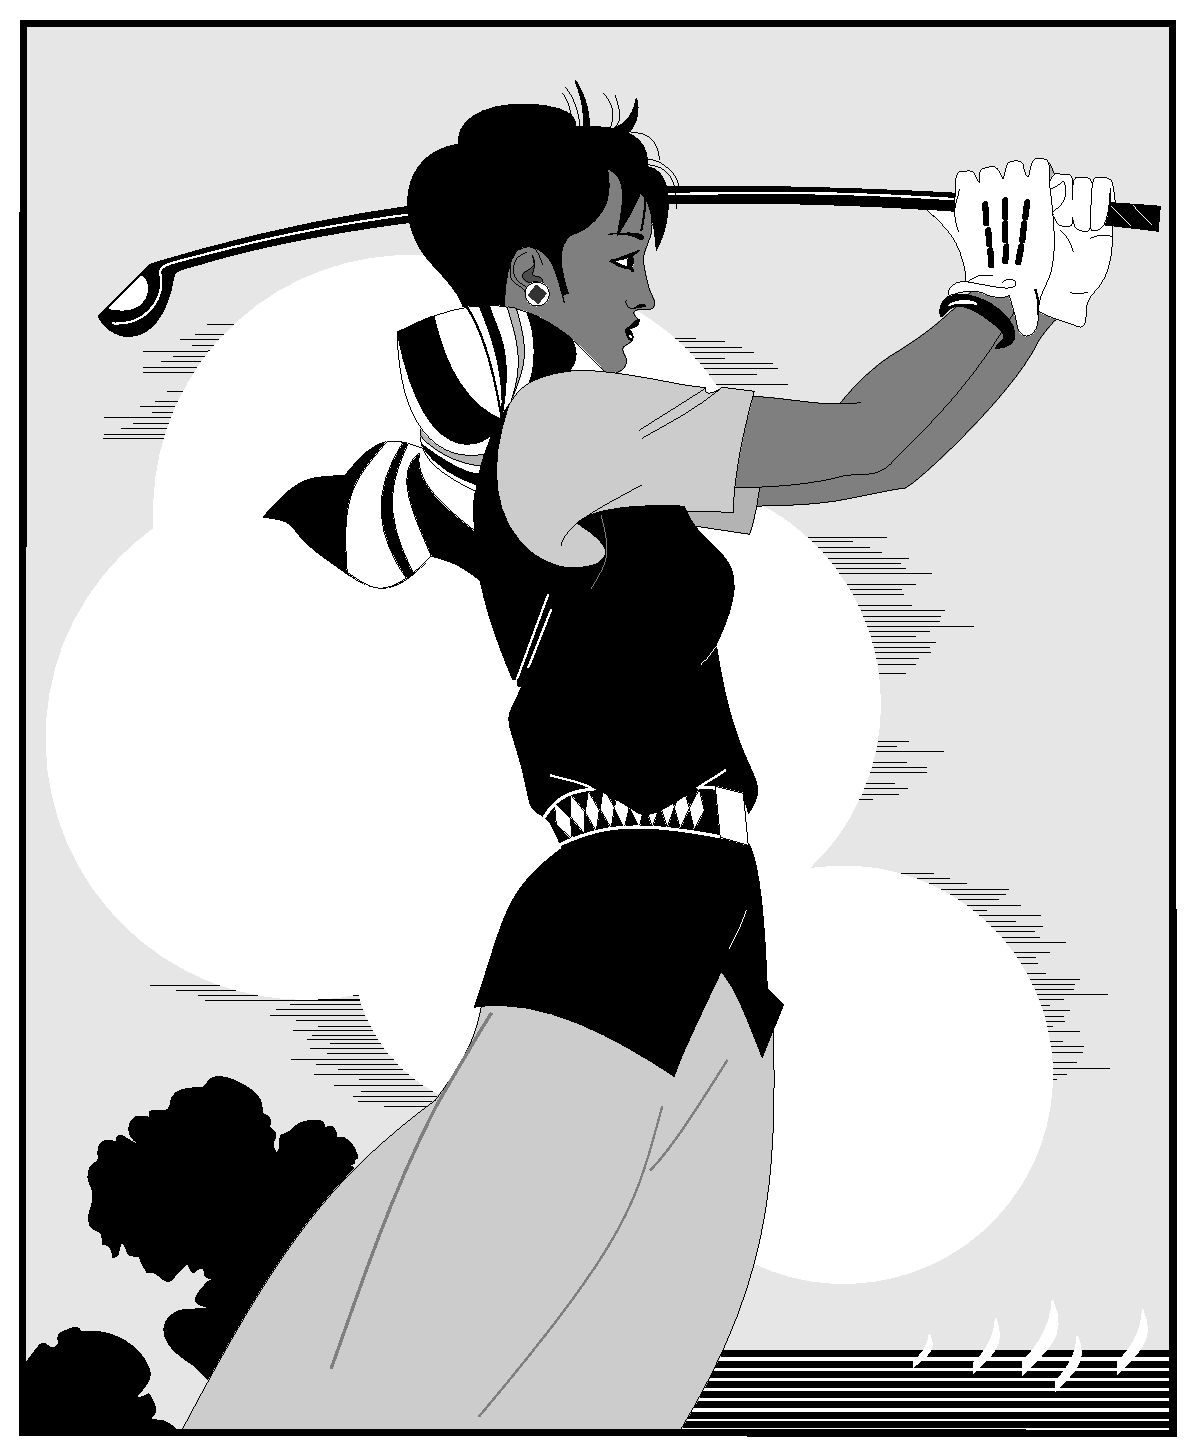
\includegraphics[width = \textwidth]{golfer}
}
\end{minipage}
\begin{minipage}{0.25\textwidth}
\centering
\subfigure[高尔夫3]{\label{Figure:Tricks:Example3:C}
  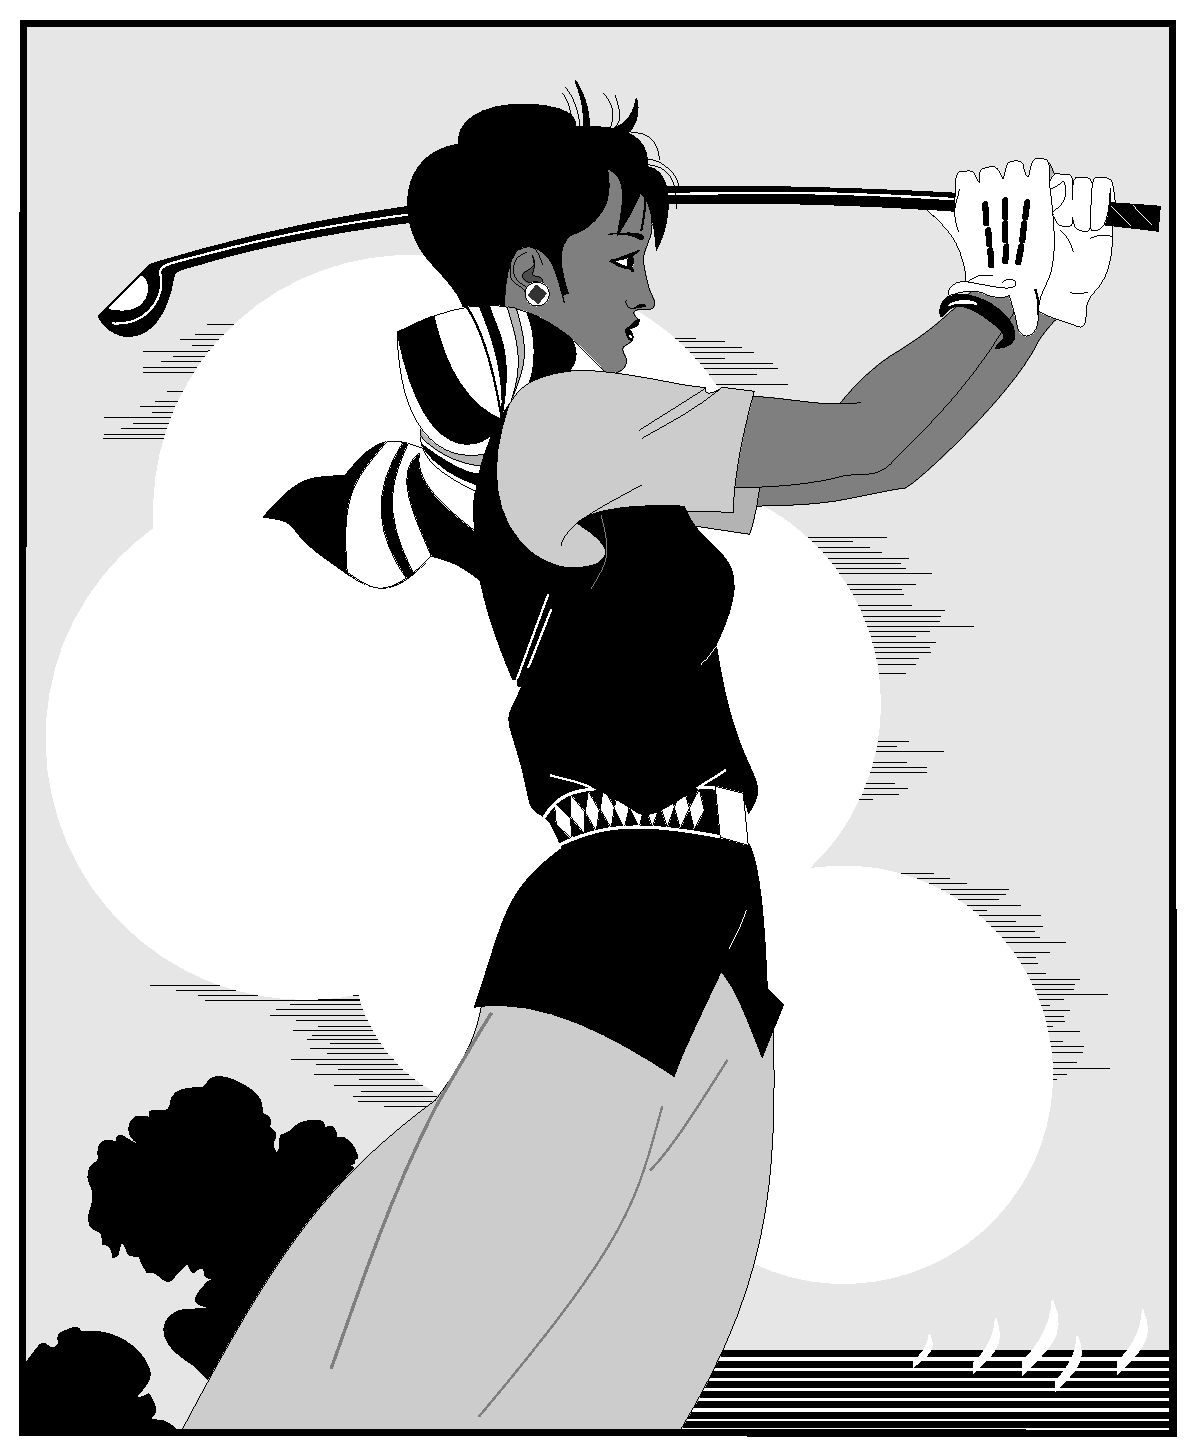
\includegraphics[width = \textwidth]{golfer}
}
\end{minipage}
\FigCaption{高尔夫}
\label{Figure:Tricks:Example3}
\end{figure}


\begin{table}[htbp]
\centering
\TabCaption{表格测试}
\label{Tricks:Tab1}
\begin{tabular}{c|c|c}
  \hline
  % after \\: \hline or \cline{col1-col2} \cline{col3-col4} ...
  方法 & 精度~(\%) & 速度~(ms) \\
  \hline
  小波变换 & $99.8$ &  20\\
  傅立叶变换 & $99.0$ & 30 \\
  \hline
\end{tabular}
\end{table}

\clearpage
\begin{longtable}{lll}
\LTCaption{中文标题短}\\
\bfseries Entity & \bfseries Unicode Name & \bfseries Unicode \\ \hline
\endfirsthead
\bfseries Entity & \bfseries Unicode Name & \bfseries Unicode \\ \hline
\endhead
\hline \multicolumn{3}{r}{\emph{Continued on next page}}
\endfoot
\hline
\endlastfoot
a&emf&bcdef\\
a&emf&bcdef\\
a&emf&bcdef\\
a&emf&bcdef\\
a&emf&bcdef\\
a&emf&bcdef\\
a&emf&bcdef\\
a&emf&bcdef\\
a&emf&bcdef\\
a&emf&bcdef\\
a&emf&bcdef\\
a&emf&bcdef\\
a&emf&bcdef\\
a&emf&bcdef\\
a&emf&bcdef\\
a&emf&bcdef\\
a&emf&bcdef\\
a&emf&bcdef\\
a&emf&bcdef\\
a&emf&bcdef\\
%a&emf&bcdef\\
\end{longtable}


\section{算法 Algorithms}
这是一个算法的例子,来自~worldguy@lilacbbs~
\begin{algorithm}
\KwIn{training samples, {$(d_i, d_j)_q$; $\mathbf{q}_i, \mathbf{q}_j \in C$, $q\in \mathbf{Q}$} }
\KwOut{parameter setting $\lambda^T$}

Initialization : set $\lambda_0=1, \lambda_i=0$, for i=$1, \dots, N$

\For{$t$=1 to $T$}
{
    \ForEach{training sample $(d_i, d_j)_q$}
    {
        \If{ $Score(q, d_j, \lambda^t) \ge Score(q, d_i, \lambda^t)$ }
        {
            \ForEach{$\lambda^t_n (n=1, \dots, N)$}
            {
                $\lambda^{t+1}_n = \lambda^t_n + \eta (f_n(q, c, d_i) - f_n(q, c, d_j))$
            }
        }
    }
}
\end{algorithm}

\subsection{公式}
\label{Tricks:Equations}

文本中的数学符号和公式用下面的方法输入:

天体力学问题所采取的一个最基本的模型就是通常所说的$N$体问题,即在一
定条件下,所研究的天体被看成质点,$N$体问题最简单的就是二体问题。在一
个天体系统中,$N$个天体往往包含$n$个大天体和$k$个小天体($N=n+k$),其中
$k$个小天体相对$n$个大天体而言小到对后者运动的影响几乎不用考虑,但$k$
个小天体之间可能相距较近,它们之间的相互作用应予考虑,这就构成了限制
性($n+k$)体问题。特别地,当$N=3,~n=2,~k=1$时,即通常所说的限制性三体问题。


最基本的数学公式,带序号的:
\begin{equation}
\ddot{\mathbf{r}}=\mathbf{F}_{0}(r)+\mathbf{F}_{\varepsilon}(\mathbf{r},\dot{\mathbf{r}},t)
\end{equation}

这是一个不带序号的例子:
\begin{displaymath}
F_{\varepsilon}/F_{0}=O (\varepsilon)
\end{displaymath}

\FloatBarrier %清除浮动体
典型的公式加符号说明的例子:

目标飞行器和追踪飞行器之间的相对运动方程为:
\begin{equation}\label{eq:1}
\ddot{\boldsymbol{\rho}}-\frac{\mu}{R_{t}^{3}}\left( 3\mathbf{R_{t}}\frac{\mathbf{R_{t}\rho}}{R_{t}^{2}}-\boldsymbol{\rho}\right)=\mathbf{a}
\end{equation}
其中:

$\boldsymbol{\rho}$---追踪飞行器与目标飞行器之间的相对位置矢量;

$\ddot{\boldsymbol{\rho}}$---追踪飞行器与目标飞行器之间的相对加速度;

$\mathbf{a}$---推力所产生的加速度;

$\mathbf{R}_{t}$---目标飞行器在惯性坐标系中的位置矢量;

$\omega_{t}$---目标飞行器的轨道角速度;

$\mathbf{g}=\frac{\mu}{R_{t}^{3}}\left(
3\mathbf{R_{t}}\frac{\mathbf{R_{t}\rho}}{R_{t}^{2}}-\boldsymbol{\rho}\right)=\omega_{t}^{2}\frac{R_{t}}{p}\left(
3\mathbf{R_{t}}\frac{\mathbf{R_{t}\rho}}{R_{t}^{2}}-\boldsymbol{\rho}\right)$---重力加速度,这里$p$是目标飞行器的轨道半通径;

公式加符号说明还可以这样:
\begin{equation}\label{eq:111}
\ddot{\boldsymbol{\rho}}-\frac{\mu}{R_{t}^{3}}\left( 3\mathbf{R_{t}}\frac{\mathbf{R_{t}\rho}}{R_{t}^{2}}-\boldsymbol{\rho}\right)=\mathbf{a}
\end{equation}
\begin{formulasymb}{式中}{-15pt}%-3pt,-20pt调与上方的间距。
  \fdesfirst{$\boldsymbol{\rho}$}{追踪飞行器与目标飞行器之间的相对位置矢量;}
  \fdes{$\ddot{\boldsymbol{\rho}}$}{追踪飞行器与目标飞行器之间的相对加速度;}
  \fdes{$\mathbf{a}$}{推力所产生的加速度;}
  \fdes{$\mathbf{R}_{t}$}{目标飞行器在惯性坐标系中的位置矢量;}
  \fdes{$\omega_{t}$}{目标飞行器的轨道角速度;}
  \fdes{$\mathbf{g}=\frac{\mu}{R_{t}^{3}}\left(
3\mathbf{R_{t}}\frac{\mathbf{R_{t}\rho}}{R_{t}^{2}}-\boldsymbol{\rho}\right)=\omega_{t}^{2}\frac{R_{t}}{p}\left(
3\mathbf{R_{t}}\frac{\mathbf{R_{t}\rho}}{R_{t}^{2}}-\boldsymbol{\rho}\right)$}{重力加速度,这里$p$是目标飞行器的轨道半通径;}
\end{formulasymb}

\subsection{定理定义}

\begin{definition}
这是定义的示例。
\end{definition}

\begin{proposition}
这是命题的示例。
\end{proposition}

\begin{lemma}
这是引理的示例。
\end{lemma}

\begin{theorem}
这是定理的示例。
\end{theorem}

\begin{axiom}
这是公理的示例。
\end{axiom}

\subsection{WinEdt的编译及其他技巧}
\label{sec:winedttricks}
~
有一文档~ WinEdt\_LaTeX\_guide.doc 简单介绍了~ WinEdt 的简单文档的编译方法,可以点击
\url{http://bbs.hit.edu.cn/bbscon.php?bid=296&id=1887&ap=719} 得到。

下面详细介绍编译按钮的含义,新手一般对这个特别好奇,
请注意这里的讲解顺序不是~ WinEdt 的默认排列顺序。
\begin{hitlist}
  \item TeX: 用来编译使用~ TeX 命令写的文档,是底层的编译系统;
  \item LaTeX: 用来编译使用~ LaTeX 命令写的文档,是目前我们使用最多的~ LaTeX2e 文档编译系统,生成~ dvi 文件;
  \item cct\& LaTeX: cct 是国内的张林波研究员开发的一个使用~ LaTeX 来处理中文文档的接口系统,
  首先把~cct 的文档由~.ctx 转换成~.tex 格式,然后调用标准的~ LaTeX 命令来生成dvi文件;
  \item PDFLaTeX: 这是类似于~LaTeX的另外一种编译系统,直接生成~pdf 文件,支持更多的~ pdf 文件特效,现在应用越来越广泛,例如做的幻灯片;
  \item BibTeX: 这个是用来处理参考文献的命令,通过它生成一个包含参考文献条目的列表~ bbl 文件供排版使用。
  \item Make Index: 这个用来生成文档的索引。
  \item TeXify: 这是几个编译命令的合集,它自动运行~ LaTeX(或pdflatex),MakeIndex 和~ BibTeX 尽可能需要的次数来生成一个
  具有排序的文献列表和交叉引用的~ dvi(pdf)文件,简化了~ dvi(pdf)文件的生成过程。
  \item CTeXify: 这个是~ CTeX 套装添加了中文支持的~TeXify 命令,可以生成中文的~ dvi(pdf) 文档。
\end{hitlist}

具体使用哪个编译按钮,和你的文档类型及包含的内容有关系。因为不同的编译命令,对于文档中的元素要求不一样,
例如,如果你引用的是~eps 图形,应该用~latex来编译,如果插入的是~pdf 图形,应该用~pdflatex 来编译。
这个解释你在前面的文档里应该也已经看到了。

\subsubsection{显示文档结构图}

WinEdt中的~gather可以收集章节标题,形成~TOC 列表,功能类似于~word 中的文档结构图,在
写大文档的时候这个功能非常有用,但是在我们的~Pluto 模板中,自定义了一些章节标题,
这些自定义标题缺省的~gather 是不识别的。TeX@lilac 提供了一种方法,在~WinEdt.gdi中定义了相关命令,
奏效。希望想使用这个功能的网友可以自己动手修改,tools 文件夹下有他修改过的~WinEdt.gdi,
网友们也可以直接使用,放到~winedt 目录下替换同名文件即可。

winEdt 的~ tree interfacezho 中也有~ TOC 这一项,这个可以通过修改 ~Winedt目录下的~WinEdtEx.ini实现。用~tools文件夹下
的~WinEdtEx.ini 替换该同名文件就可以。

另外这些自定义的命令在编辑状态下不能像缺省命令一样高亮,如果能高亮就好了,TeX 同样找到了自己定义的方法,
在~winedt 菜单~ option/highlighting/switches 修改,tools 文件下~ Switches.dat 是他已
定义好的,可以在上述菜单位置使用对话窗顶部的~``Load from'' 按钮加载。

\subsection{生成图的常见方式}

在~latex 文档编写过程中,常用的图形格式是~ eps 和~ pdf 。

pdf 文件生成,可以用很多软件生成,例如~adobe acrobat 、pdffactory、pdf xchange 等。
这里推荐~ acrobat (注意不是~ acrobat  reader),因为它安装后生成一个~ pdf 打印机,
任何一个文档都可以通过这个打印机生成~pdf 文件,更主要的功能是对~ pdf 文件阅读编辑。
pdf 文件可以在~acrobat 里进行裁剪~ (documents,crop pages...),取出部分页面。它还支持
直接另存为~ eps 文件的功能。所以,有了~acrobat 软件,几乎所有的图形处理问题都可以解决。
不过这个软件是商业软件。

可用于~latex 的作图软件比较多,所有的作图软件:~visio,~ coraldraw,~ photoshop,~ gnuplot 生成的图
都可以通过上面的方法转换成~eps 或~pdf 文件。另外,还有很多专门为~latex 开发的作图软件,
有通过命令的形式生成图的,例如~metapost,~pstricks,~asymptote,~pgf/tikz 等,也有简单的
具有作图界面的软件,例如~Dia,~winfig,~gclc 等。  总体上来讲,这些软件功能相对比较简单,做出的图也都很漂亮,但是都没有微软的
~visio 软件功能强大,所以对于入门者最好先用~visio 来作图。

对于插图的命令,王磊的中文版插图指南已经很详细了,这里不再介绍,请翻阅该书。

\subsection{快速插入图表}

对于图表等环境的插入,WinEdt 提供了很体贴的方法。只要选择工具栏的图片和表格按钮,就可以
插入一段完整的图表命令,你需要的只是把其中的星号换成自己的东西就可以了。
WinEdt还提供了一个宏,GUI 方式完成图的插入过程,选项更多,也更方便。
有时候,感觉表格比较复杂,不容易用~LaTeX 写命令,可以尝试一下 ~xl2latex 2.0 这个~ excel
输出表格为~LaTeX 代码的宏。首先在~excel 里生成表格,然后运行一下宏,就生成了表格的~LaTeX 代码。
模板的~edittools 目录下提供了这一文件。

\subsection{更多技巧及别人入门心得}
更多的入门技巧,可以参考紫丁香TeX版的置底的帖子~\href{http://bbs.hit.edu.cn/bbscon.php?board=TeX&id=2038&ftype=11}{版面部分问题导航(主要是面向新手)}。

\section{模板使用说明}

本模板是维护中的~v0.2 版本,也是第二个公开发布的版本,对照着~2006 年~5 月开题的一个~word 样本
制作,目前没有已发现的问题存在,打印效果和~Word 样本差不多。如果发现存在问题或者提出改进建议,请反馈到紫丁香~bbs 的~TeX 版。:-)

注意:在使用之前请打开目录下的~``读我.txt'' ,这里有几点附加的注意选项,以后会加到模板的使用说明里去的。

本版本的说明文档由于时间关系,还没有做出来,不过如果你以前接触过~LaTeX,相信很快就会上手的。:P

\section{模板升级记录}
\subsection{v0.11 第一个公开发布的版本}
在哈尔滨工业大学硕博士学位论文模板(SVN仓库版本150,介于1.8rc1和目前未发布的1.8rc2之间)的基础上,LaTeX@lilac
制作了工大的研究生硕博士开题报告模板。0.11 版是对照着~2006 年~5 月开题的一个~word 样本(b5纸型)制作,目前没有已发现的问题存在,打印效果和~Word 样本差不多。

\subsection{v0.2 当前发布的模板版本}
将开题模板版本控制系统内部SVN~195 版本定为~v0.2,公开发布。本版本的维护者为~LaTeX 和 luckyfox。 本版本的改动主要有以下几个方面。

\subsubsection{bugs修正}
\begin{hitlist}
  \item 调整了``参考文献''的格式。
  \item 修正了图表公式的编号,把章编号去掉。
  \item 调整了内封中"说明"的间距,有时候字体找不到,主板蜂鸣器响。加一个~\verb|\hfill| 自动调节一下。
  \item 修正定理的定义,定理后面不用冒号。
  \item 图形英文标题 缩写 由 ``Fig'' 改为``Fig.''。
  \item 调整 cmap 宏包的引用位置,适应 miktex 2.5。
\end{hitlist}


\subsubsection{功能增强}
\begin{hitlist}
  \item 在原来~b5 纸型的基础上增加了~a4 纸型,供用户选择。推荐使用~a4 纸型。a4 版本的正文字号与博士论文规定一致,版芯比博士论文要大,可能是因为开题报告不用装订吧。
  \item 参考最新的硕士开题封面,提供对硕士开题的支持。
  \item 增加了对 winedt5.5 中自定义命令在 tree 和 gather 中的 toc 的支持。
\end{hitlist}


\subsubsection{文档说明}
 \begin{hitlist}
   \item 调整``模板使用说明''一节的位置;
   \item 增加模板升级记录;
 \end{hitlist} 